The output of the data-processing pipeline described in \sref{data} is the data
set $X$, which is split into three parts: $X_1$ is for the training stage, $X_2$
for the validation stage, and $X_3$ for the testing stage. In what follows, we
elaborate on the processes that are taking place during these three stages of
working with the model presented in \sref{model}.

\subsection{Training} \slab{training}
The model in \sref{model} has a large number of parameters that have to be
learned during training; they are primarily various wights and biases inside the
model's layers. For this purpose, $X_1$ is utilized. The training is undertaken
via backpropagation through time using stochastic gradient descent
\cite{goodfellow2016} whose objective is to minimize a certain loss function,
which we shall specify shortly. The variant of gradient descent that we use is
Adam \cite{kingma2014}, which is an adaptive optimization method. There are two
aspects to be discussed about training.

\begin{figure}[t]
  \centering
  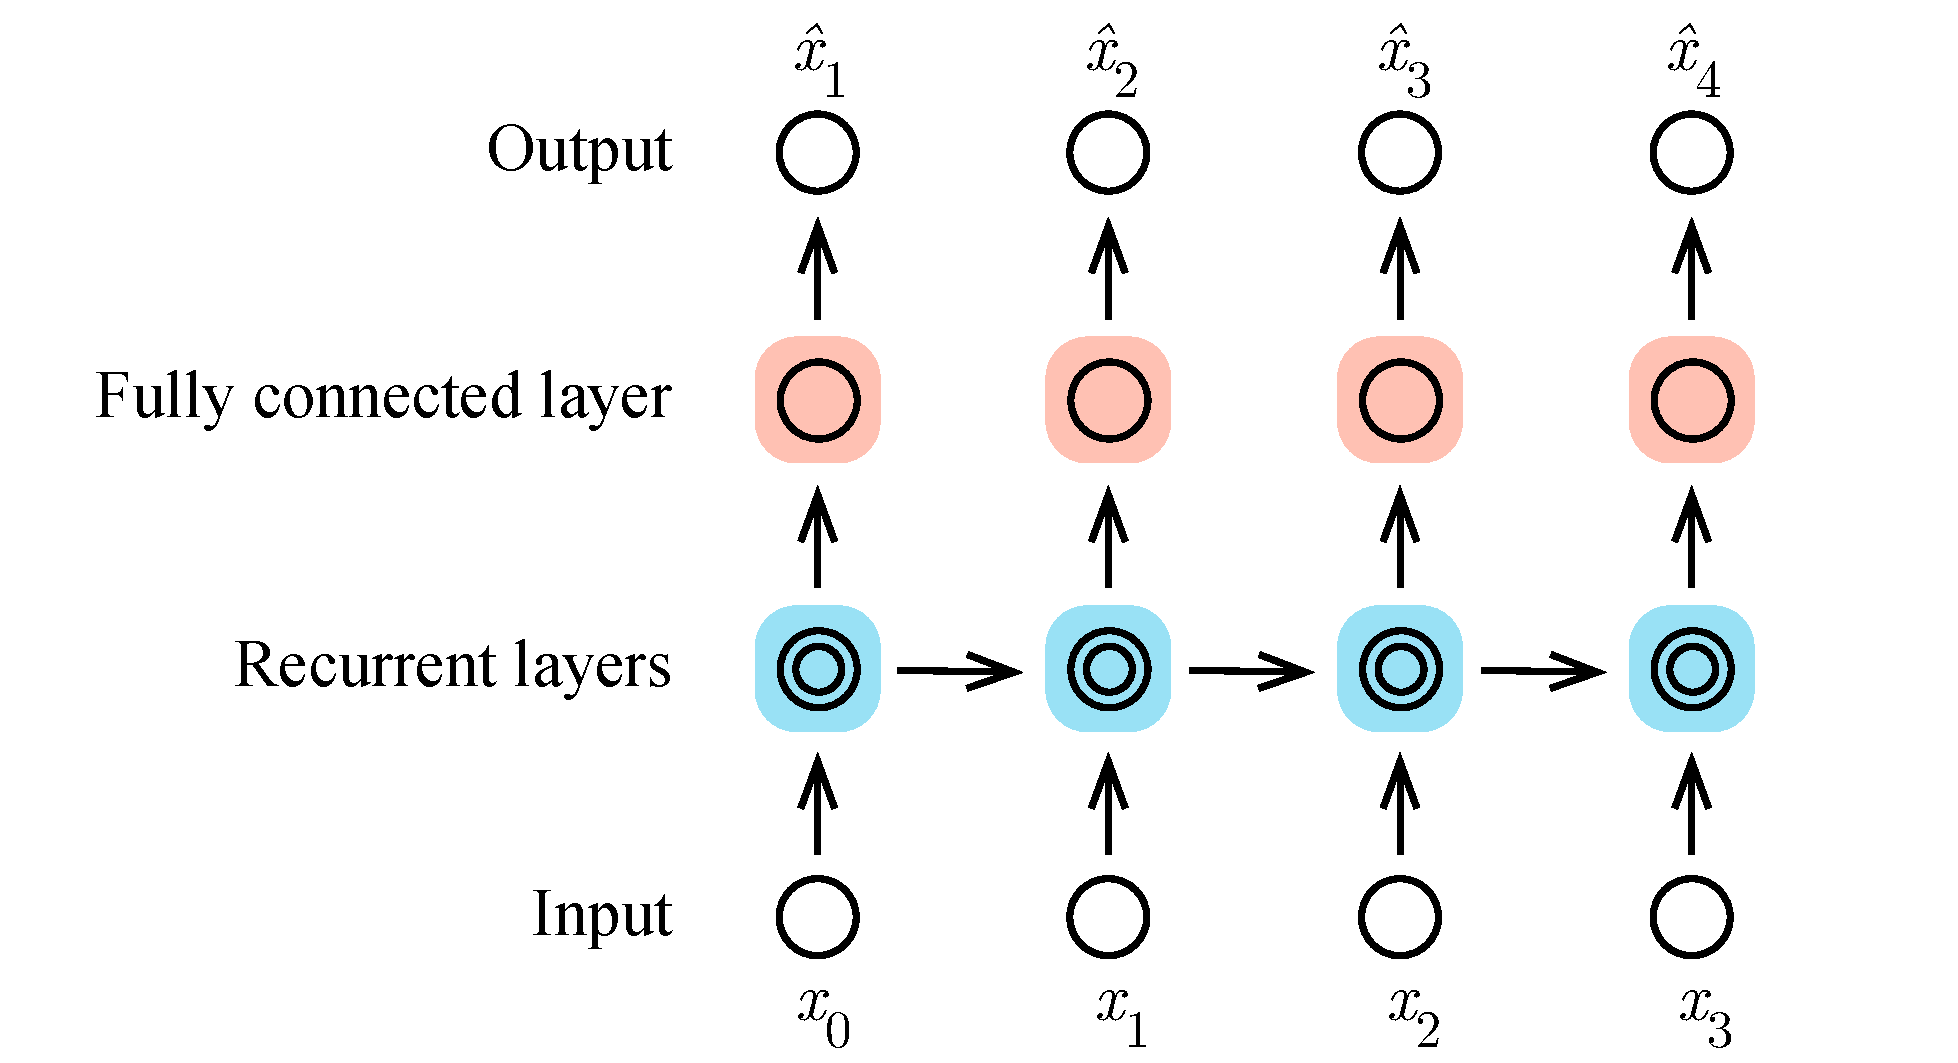
\includegraphics[width=1.0\columnwidth]{include/assets/figures/unroll.pdf}
  \vspace{-1.5em}
  \caption{An example of dynamic unrolling during the model's usage.}
  \vspace{-1.5em}
  \flab{unroll}
\end{figure}

The first concerns the way a single resource-usage trace is fed into the model.
First, note that a trace has multiple data points ($l_i > 1$), and that two
traces are of different lengths in general ($l_i \neq l_j$) since the execution
times of different tasks can differ substantially. All the points of a trace are
fed in one pass using a technique called dynamic unrolling. An illustration for
$l_i = 4$ is given in \fref{unroll}, in which the representation in \fref{model}
has been simplified even further and put on a side. It can be seen that the
model has been replicated as many times are there are data points in the trace.
However, it is still the same model, and all the replicas share the same
parameters. It can also be seen in \fref{unroll} how information flows from one
step to the next, which is what makes the model recurrent.

Now, it is not efficient to feed only one trace at a time due to the inevitable
overhead imposed by the computations involved. Therefore, these computations
should be performed in batches whenever possible. Since $l_i \neq l_j$ in
general, it is not possible to stack multiple arbitrary traces into a single
tensor directly. In order to circumvent this problem, we reside to bucketing.
Specifically, each read trace is put into one of many queues depending on its
length. When a queue accumulating traces of some length $l$ has collected the
desired number of traces---denoted by $b$ and referred to as the batch size---it
emits a tensor of size $b \times l \times d$ to be further consumed by the
model.

The loss function that is being minimized during training is the mean squared
error of one-step predictions over the whole batch. The correct prediction for
the very last time step, which goes beyond the time window of the traces in
question, is assumed to be zero. To give an example, in \fref{unroll},
$\hat{x}_{i4}$ has no $x_{i4}$ to be compared with; $x_{i4}$ is assumed to be
zero.

The above workflow has been found to significantly speed up the training
process and is highly recommended.

\subsection{Validation}
As it is the case with all nontrivial machine-learning models, the one presented
in \sref{model} has a number of hyperparameters. Examples include the number of
cells (recurrent layers), number of units per cell, and probability of dropout.
Unlike (ordinary) parameters, which are to be optimized during training (see
\sref{training}), hyperparameters are to be set prior to training, and they are
typically kept unchanged thereafter. From the examples given, it is apparent
that the impact of hyperparameters is profound. Therefore, they should be
carefully configured.

The validation set $X_2$ is used to assess the performance of the model trained
(using $X_1$ as usual) under different configurations of the model's
hyperparameters. The trained model that has the best performance on $X_2$ is
then chosen as the final one.

Despite all the techniques employed to speed up training, it is still an
expensive operation. As a result, brute-force search in the space of
hyperparameters for the best configuration is impractical; a certain intelligent
strategy should be followed.

In our workflow, we use the Hyperband algorithm \cite{li2016}. Instead of
adaptively choosing configurations to try---which is the case with other
techniques---it adaptively allocates resources, such as the number of training
steps, to configurations chosen at random, which has been shown to be a very
efficient strategy. In particular, the algorithm allows one to save a lot of
compute power, which otherwise would be burnt in vain evaluating overtly
inadequate configurations of hyperparameters.

\subsection{Testing}
In order to have a long-range prediction (multiple steps ahead), we use
refeeding: the predicted value $\hat{x}_{i,k + 1}$ is fed into the model as if
it was the actual resource usage $x_{i,k + 1}$ at step $k + 1$, which is not
yet known at time step $k$. The process continues until all the desired $h$
future values are estimated.
